    \subsection*{Example of Activation Functions}
    
        So, let's look at some possible \textbf{activation} functions:
        
        \begin{itemize}
            \item \vocab{Identity} function $z$:

                \begin{equation}
                    f(z) = z
                \end{equation}

                \begin{figure}[H]
                    \centering
                    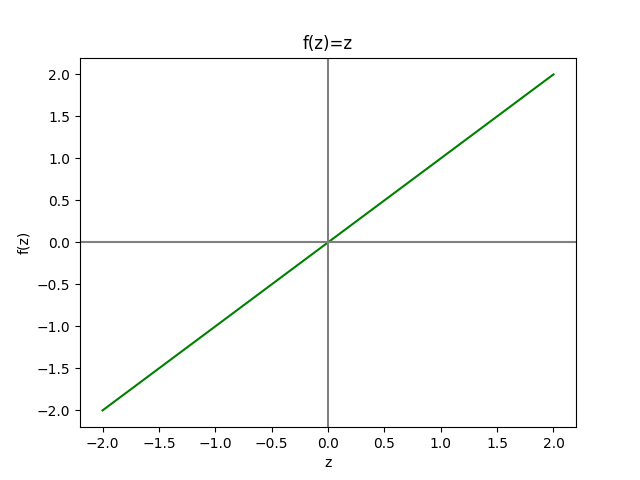
\includegraphics[width=60mm,scale=0.4]{images/nn_images/identity_fn.png}
                \end{figure}
                

                \begin{itemize}
                    \item This function is called an \textbf{identity} function because it "preserves the identity" of the input: the output is the same.

                    \item This is an example of a \textbf{linear} function.
                        \begin{itemize}
                            \item As we described in the last section*, linear activation can't make our model more \textbf{expressive}.
                            \item So, we \textbf{almost never} use it (or any other \textbf{linear} function) as an activation for a \textbf{hidden} layer.
                        \end{itemize}
                    \item We mainly use this an \textbf{output} activation function: it allows our final output to be any real number.
                        \begin{itemize}
                            \item This is a good activation function for a \textbf{regression} model, which returns a \textbf{real} number.
                            \item It's a simple function, that can return \textbf{any} real number. By constrast, sigmoid and ReLU both have \textbf{limited} output ranges.
                        \end{itemize}
                \end{itemize}

            
            \item \vocab{Step} function $\text{step}(z)$:
            
                \begin{equation}
                    \text{step}(z) 
                    =
                    \begin{cases}
                      1 & \text{if $z \geq 0$}\\
                      0 & \text{if $z < 0$}
                    \end{cases}
                \end{equation}
                
                \begin{figure}[H]
                    \centering
                    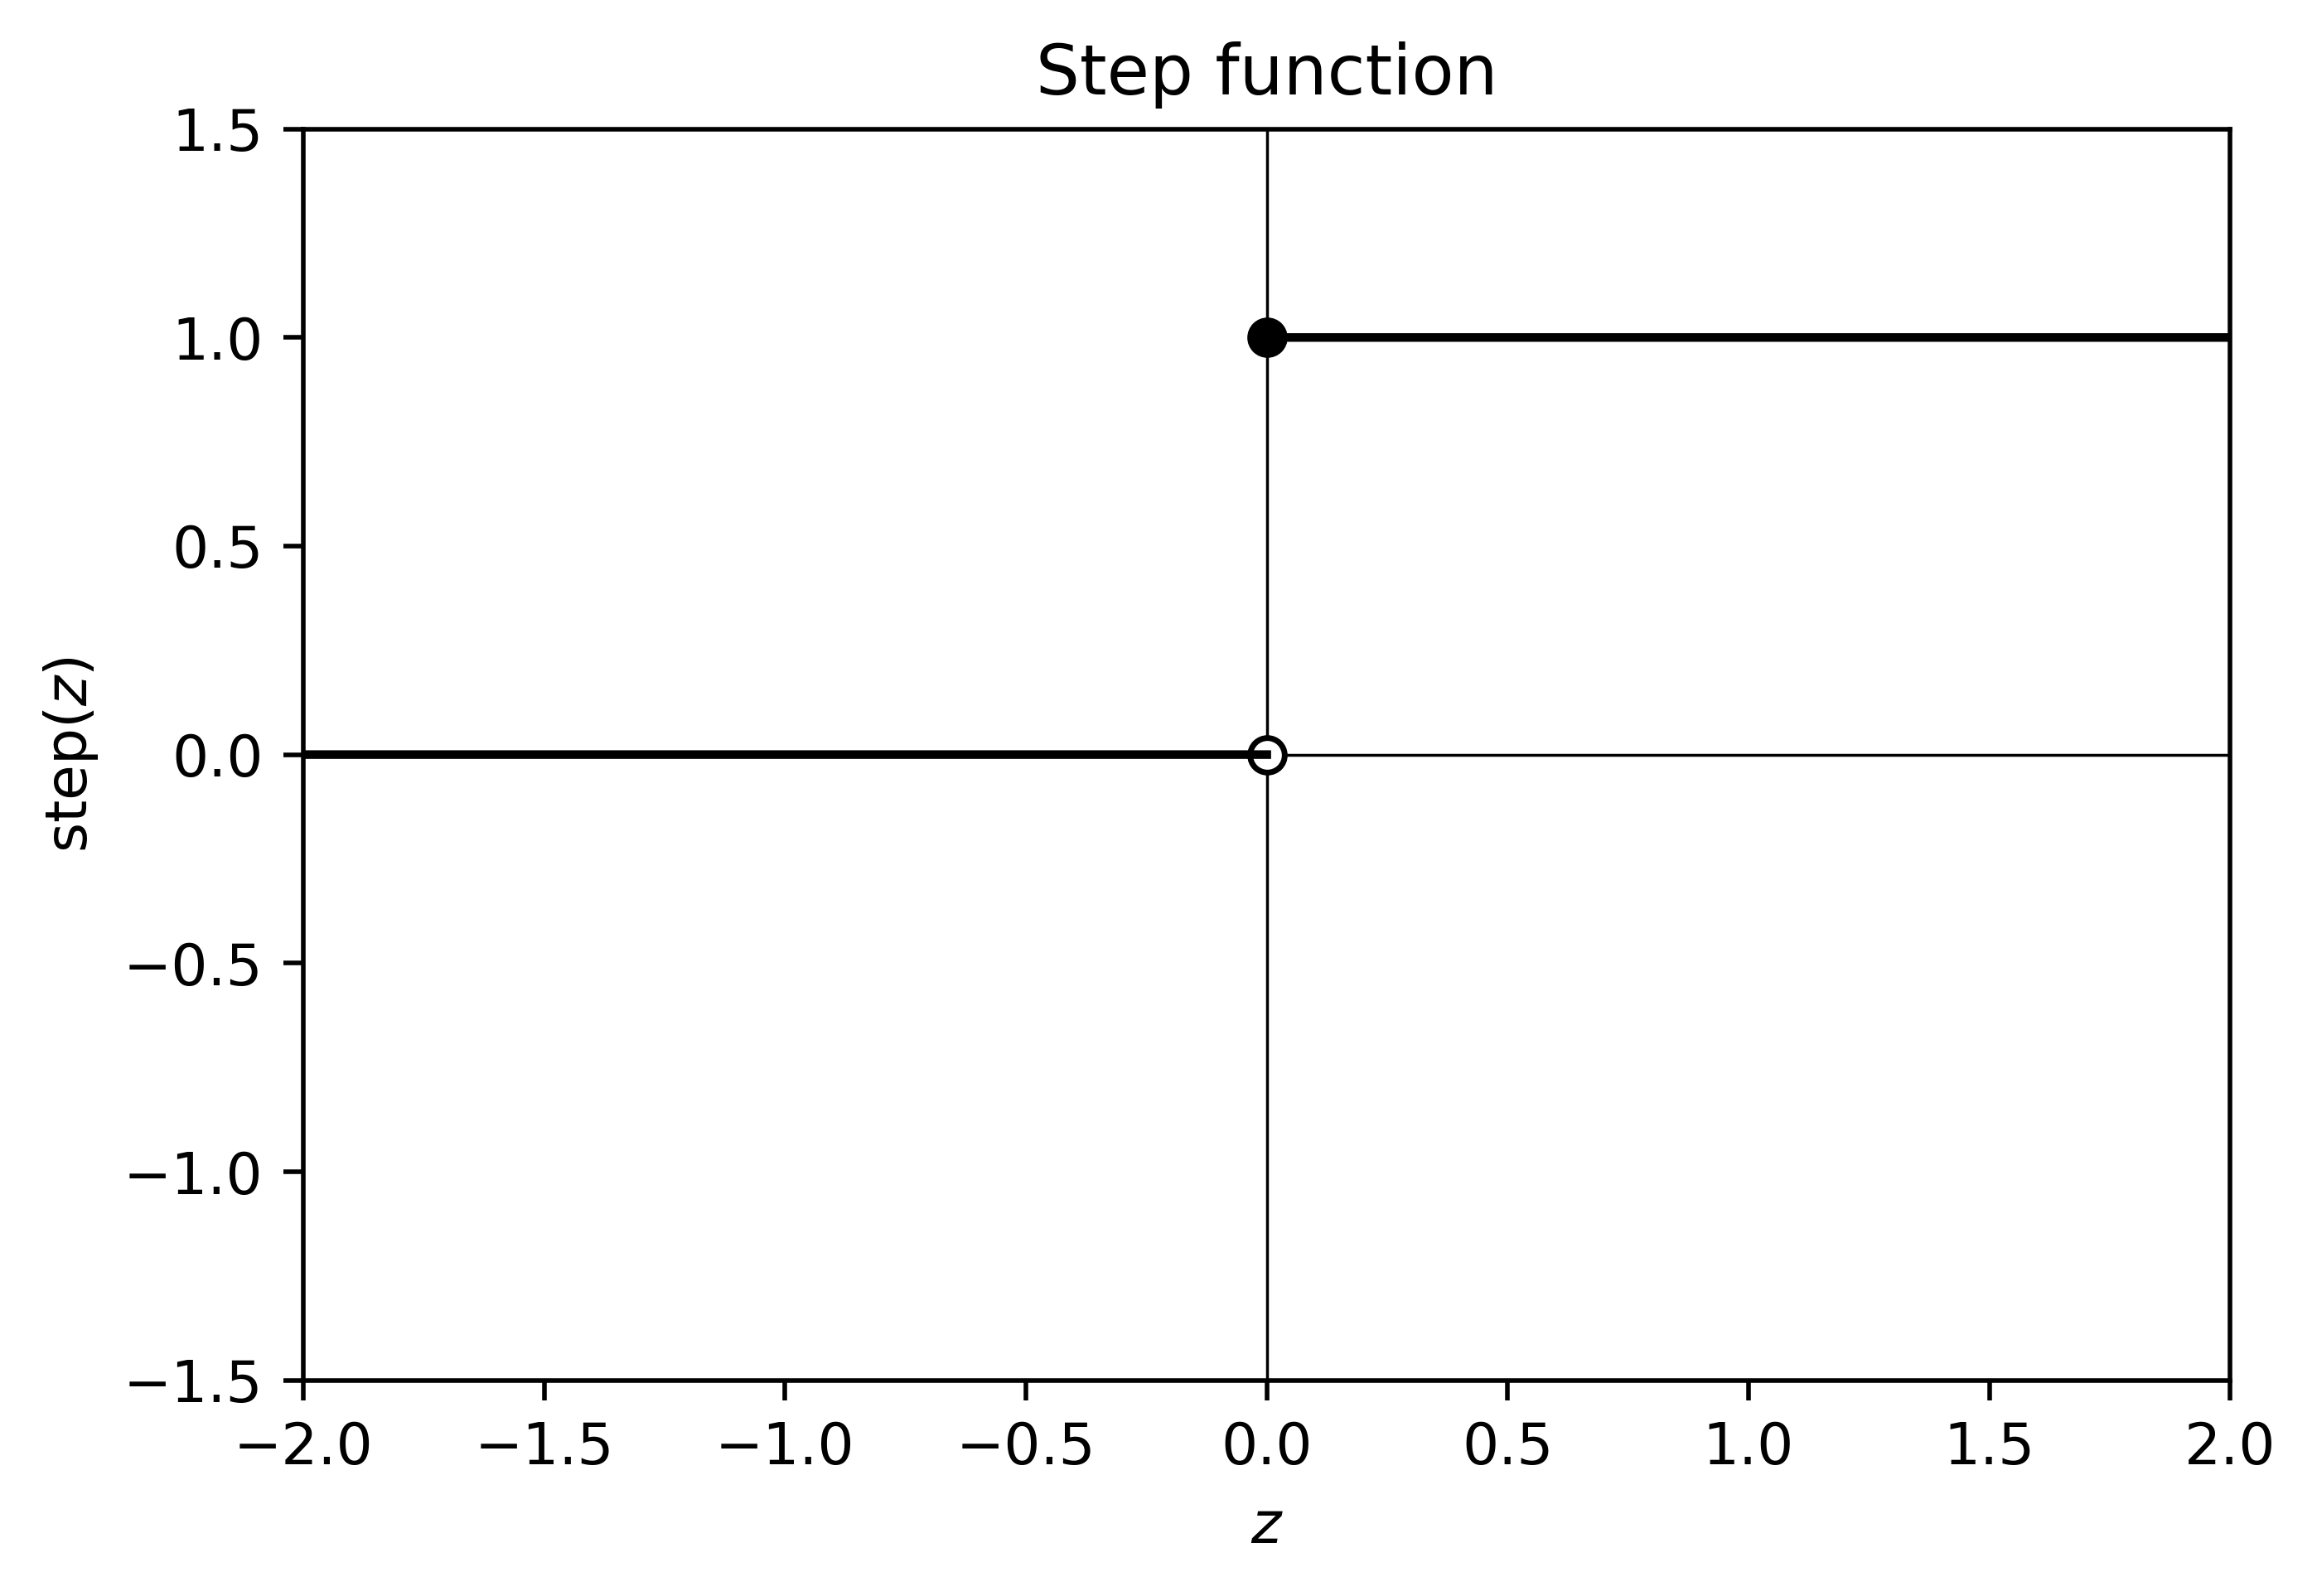
\includegraphics[width=60mm,scale=0.4]{images/nn_images/step_fn.png}
                \end{figure}
                
                \begin{itemize}
                    \item This function is basically a \textbf{sign} function, but uses $\{0, 1\}$ instead of $\{-1, +1\}$.
                    
                    \item Step functions were a common early choice, but because they have a \textbf{zero} gradient, we can't use \textbf{gradient descent}, and so we basically \textbf{never} use them.
                        \note{Same reason we replaced the sign function with sigmoid.}
                \end{itemize}
            
            
            \item \vocab{Rectified Linear Unit} ReLU$(z)$:
            
                \begin{equation}
                    \text{ReLU}(z) 
                    =
                    \max(0,z)
                    =
                    \begin{cases}
                      z & \text{if $z \geq 0$}\\
                      0 & \text{if $z < 0$}
                    \end{cases}
                \end{equation}
                
                \begin{figure}[H]
                    \centering
                    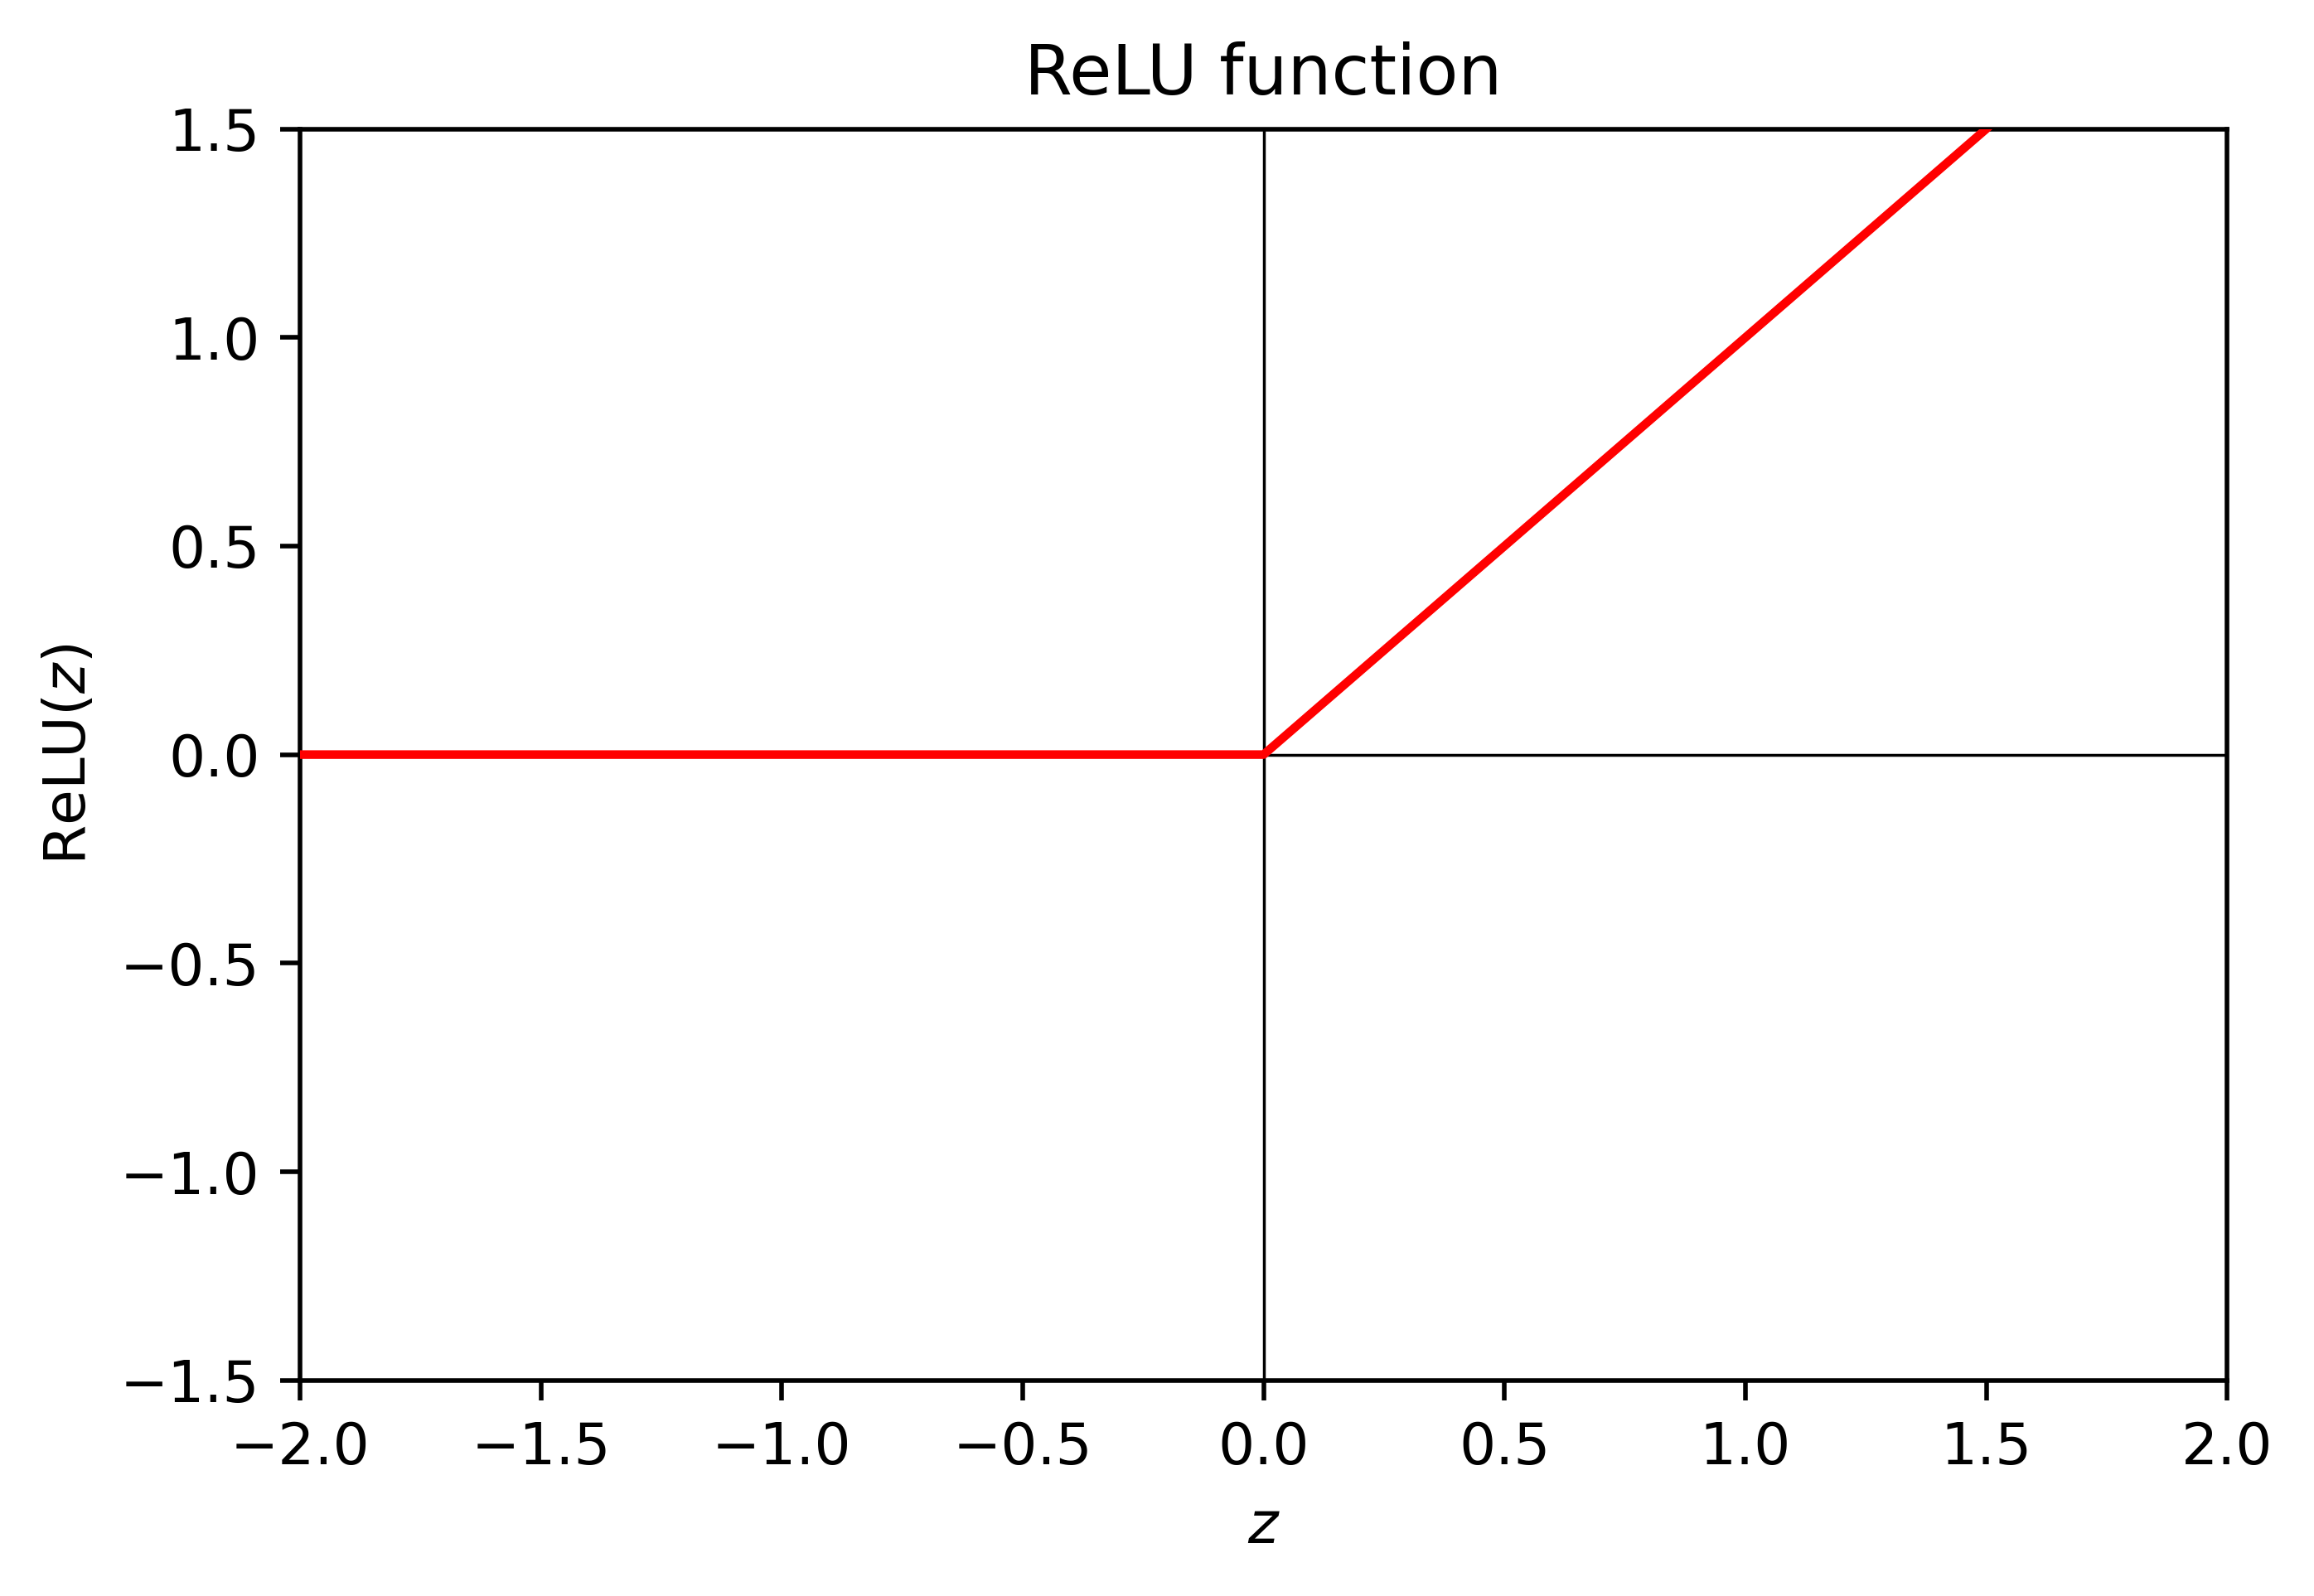
\includegraphics[width=60mm,scale=0.4]{images/nn_images/relu_fn.png}
                \end{figure}
                
                \begin{itemize}
                    \item This is a very \textbf{common} choice for activation function, even though the derivative is undefined at 0.
                    
                    \item We specifically use it for internal ("\textbf{hidden}") layers: layers that are neither the \textbf{first} nor \textbf{last} layer.
                        \note{They're "hidden" because they aren't visible to the input or output.}
                \end{itemize}
            
            
            \item \vocab{Sigmoid} function $\sigma(z)$:
            
                \begin{equation}
                    \sigma(z) = \frac{1}{1+e^{-z}}
                \end{equation}
                
                \begin{figure}[H]
                    \centering
                    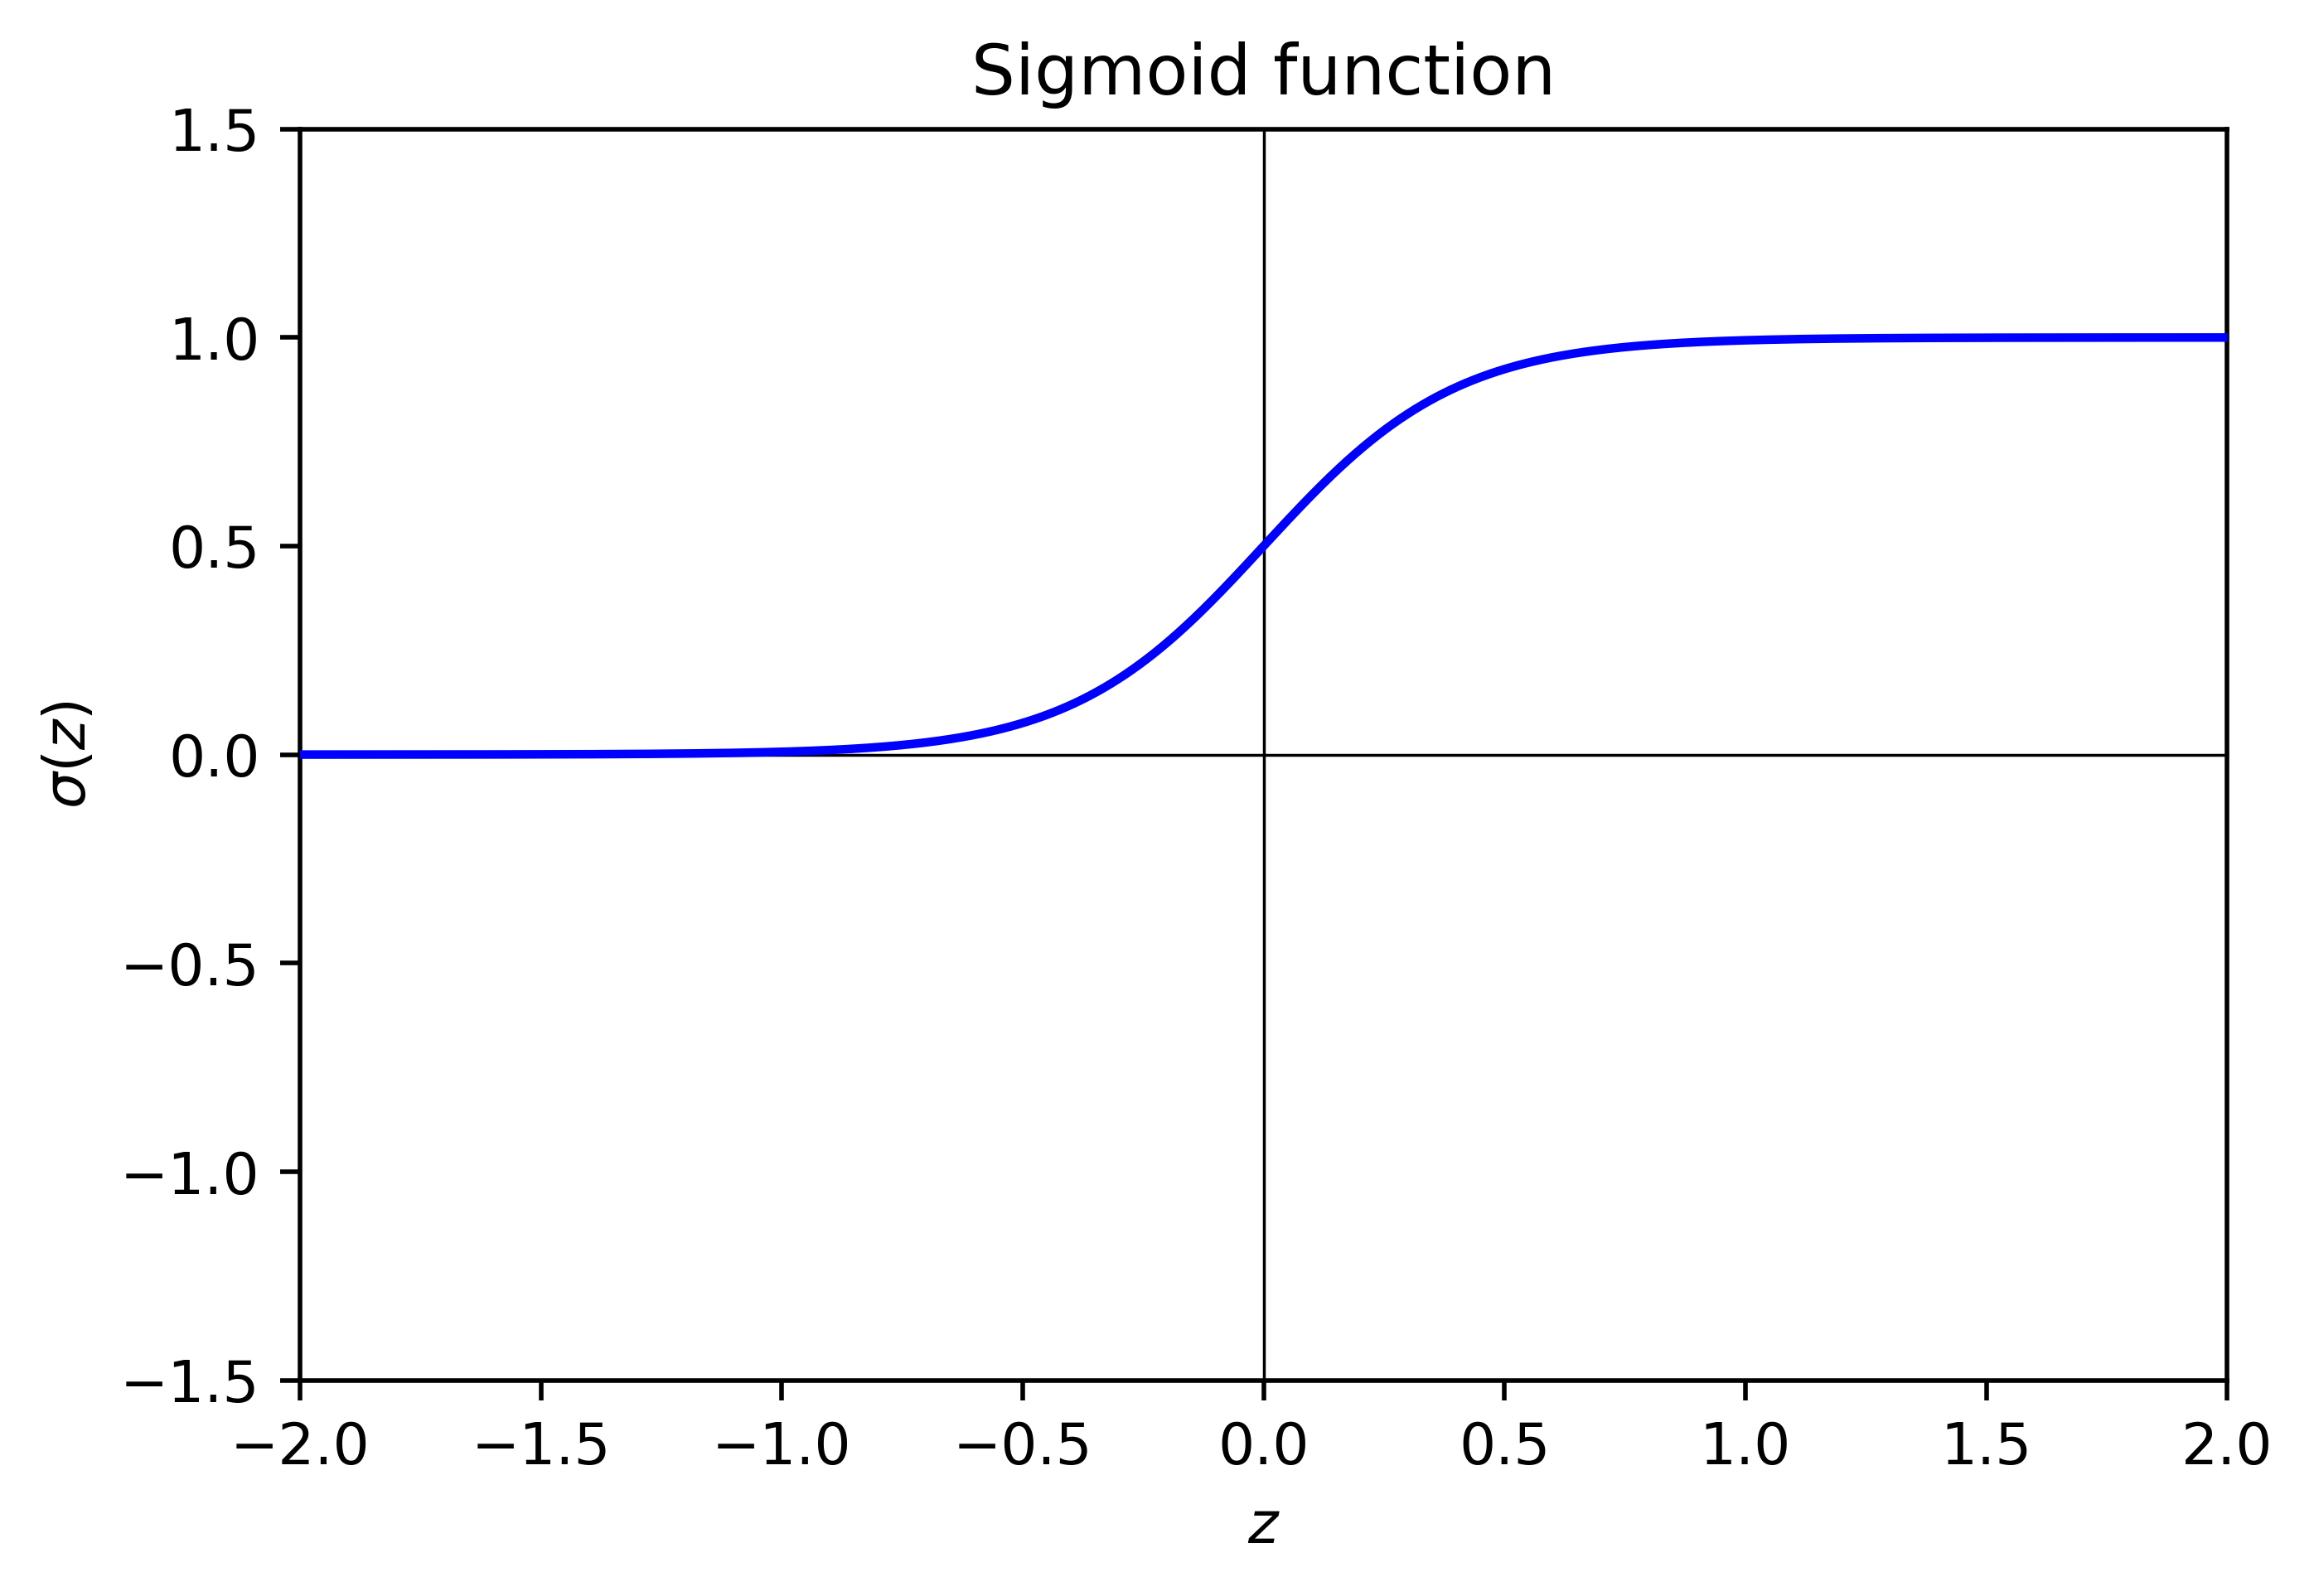
\includegraphics[width=60mm,scale=0.4]{images/nn_images/sigmoid_fn.png}
                \end{figure}
            
                \begin{itemize}
                    \item This is the \textbf{activation} function for our \textbf{LLC} neuron from before.
                    
                    \item Just like LLC, it's useful for the \textbf{output neuron} in \textbf{binary classification}.
                    
                    \item Can be interpreted as the \textbf{probability} of a positive ($+1$) binary classification.

                    \item We can also use this for multiclass when classes are \textbf{NOT} disjoint: we use one sigmoid per class.
                        \begin{itemize}
                            \item Each sigmoid tells us how likely the data point is to be in that class.
                        \end{itemize}
                \end{itemize}
                
            \item \vocab{Hyperbolic Tangent} $\tanh(z)$:    
                
                \begin{equation}
                    \tanh(z) = \frac{e^z - e^{-z}}{e^z + e^{-z}}
                \end{equation}
                
                \begin{figure}[H]
                    \centering
                    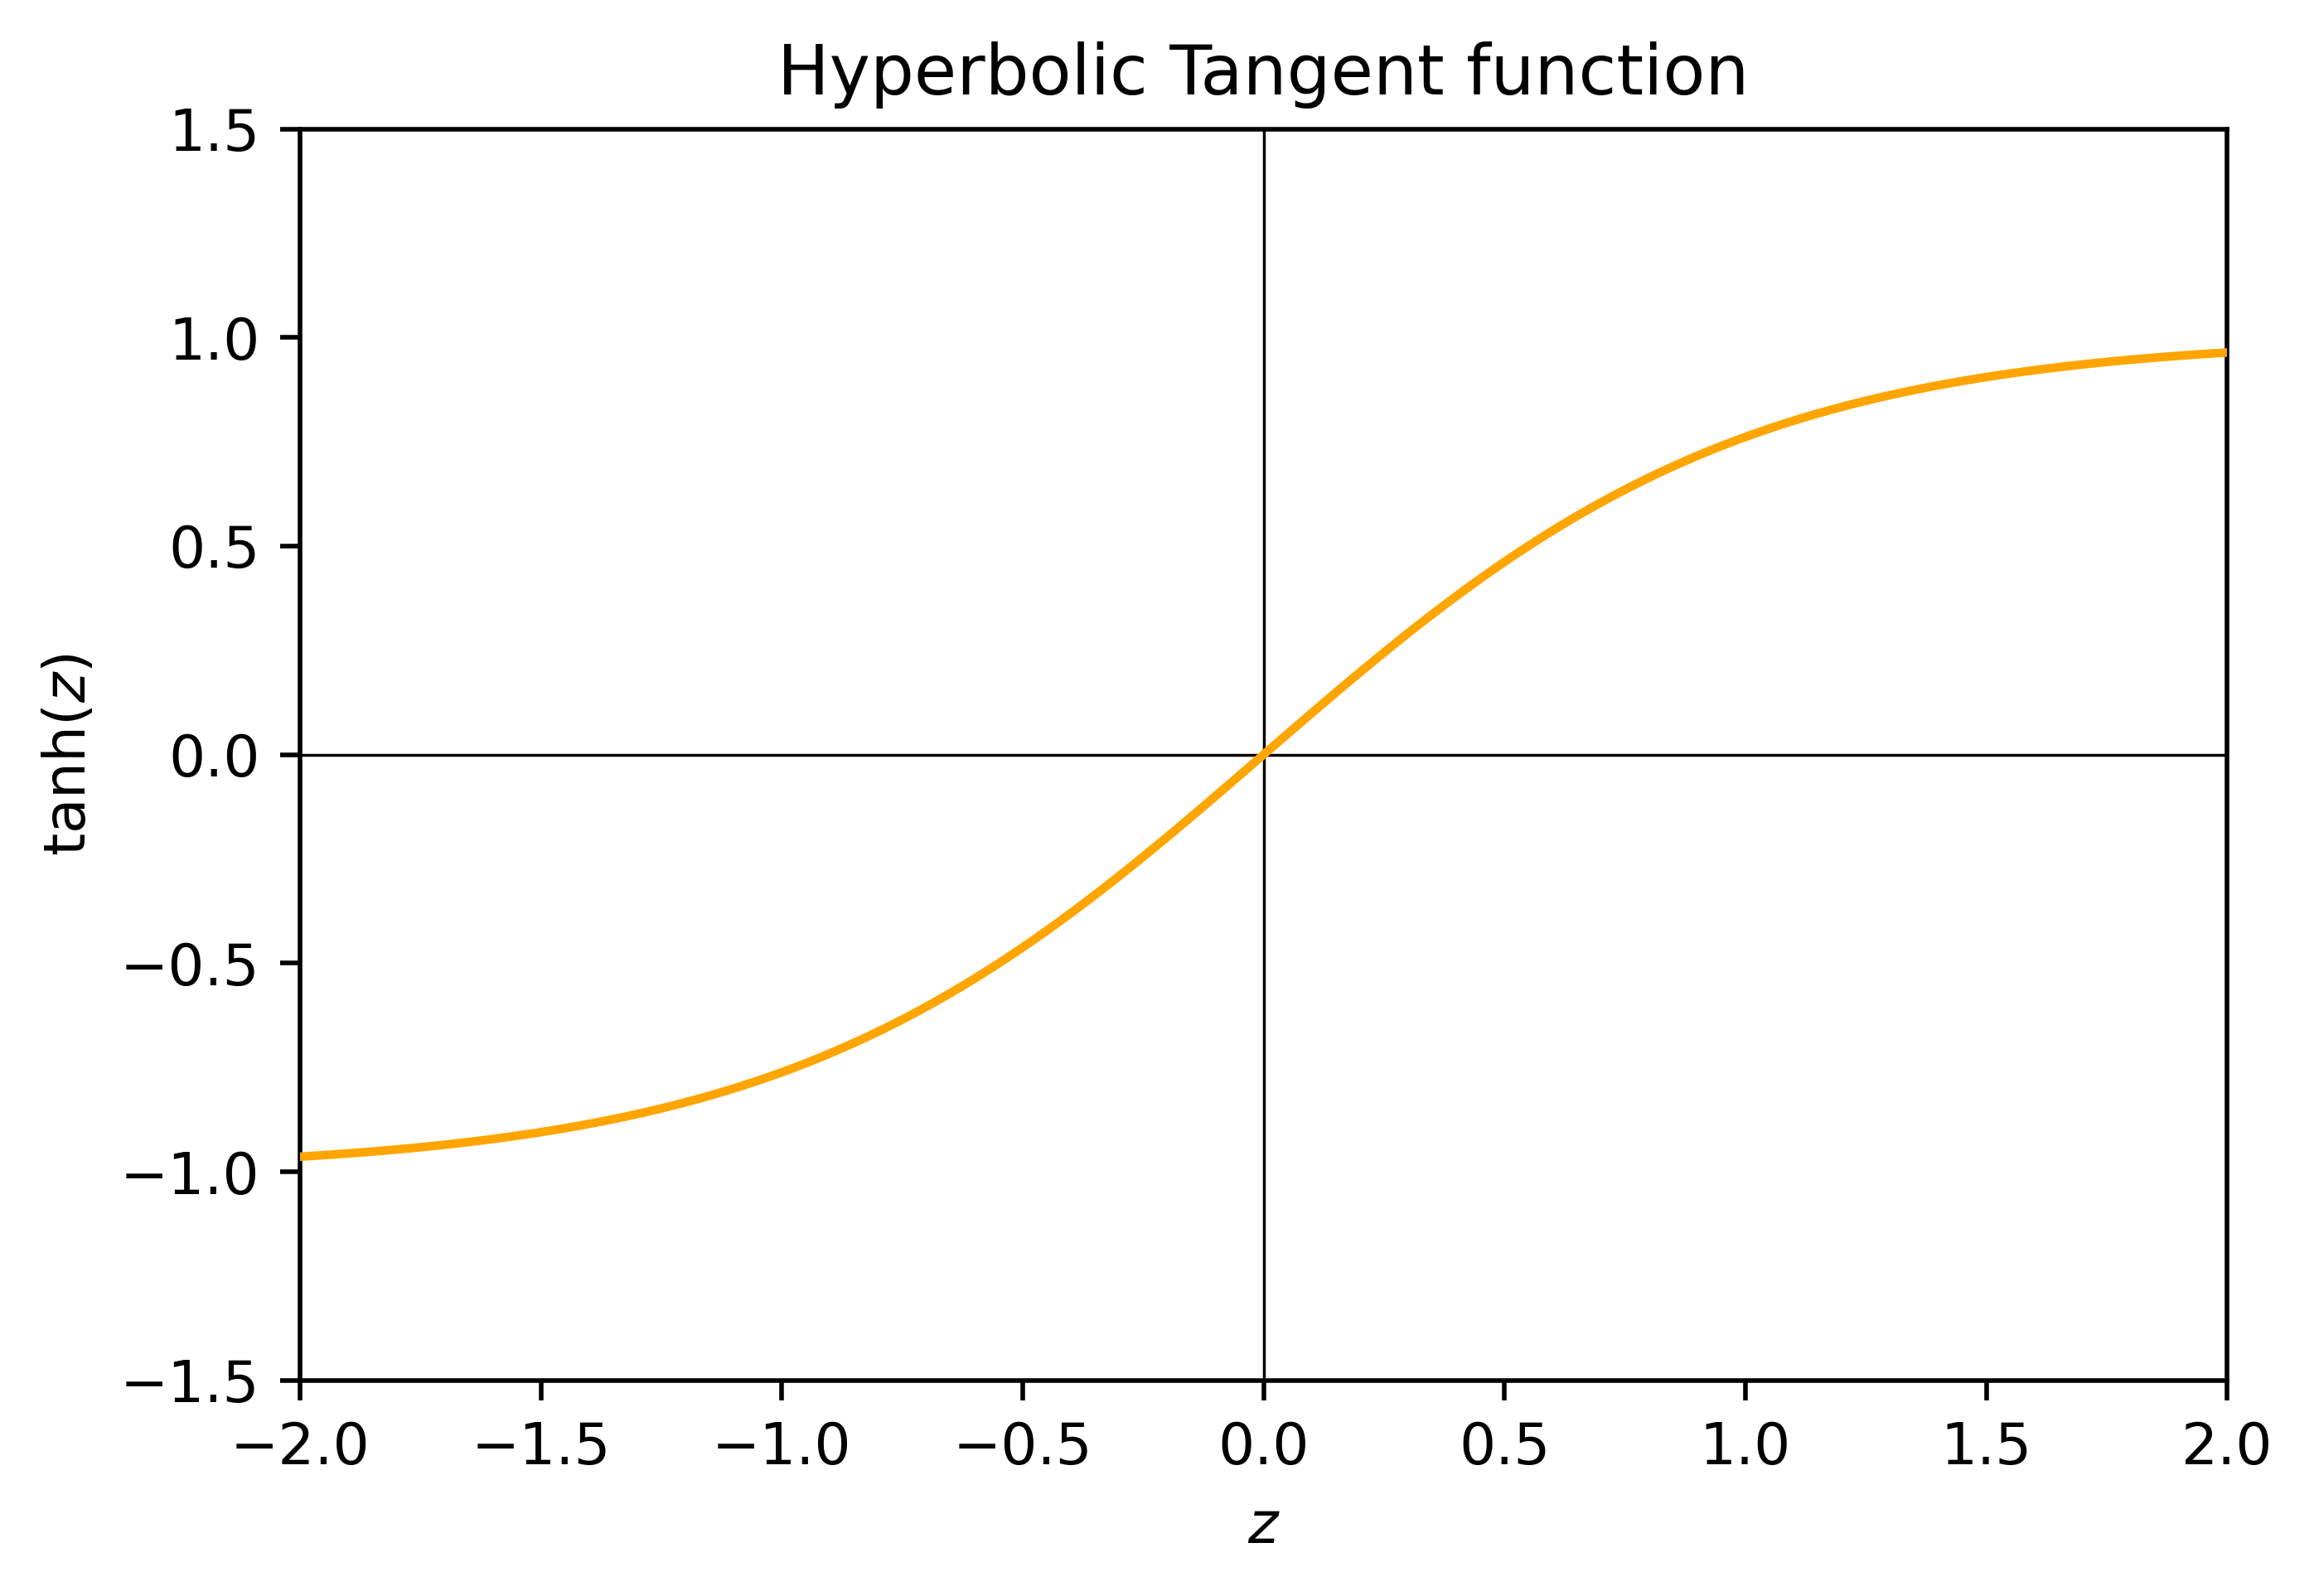
\includegraphics[width=60mm,scale=0.4]{images/nn_images/tanh_fn.png}
                \end{figure}
                
                \begin{itemize}
                    \item This is function looks similar to sigmoid over a different \textbf{range}.
                    
                    \item Unfortunately, it will not get much use in this class.
                \end{itemize}
                
            \item \vocab{Softmax} function softmax$(z)$:
                
                \begin{equation}
                    \text{softmax}(z) =
                    \begin{bmatrix}
                        \exp(z_1) / \sum_{i} \exp(z_i) \\
                        \vdots \\
                        \exp(z_n) / \sum_{i} \exp(z_i)
                    \end{bmatrix}
                \end{equation}
                
                \begin{itemize}
                    \item Behaves a like a \textbf{multi-class} version of \textbf{sigmoid}.
                    
                    \item Appropriately, we use it as the \textbf{output neuron} for \textbf{multi-class} classification.
                    
                    \item Can be interpreted as the \textbf{probability} of our $k$ possible classifications.
                        \begin{itemize}
                            \item "Disjoint" probability: each option is separate. Sum of the rows adds up to 1.\\
                        \end{itemize}
                \end{itemize}
        \end{itemize}
        
        \begin{concept}
            For the different \vocab{activation functions}:
            
            \begin{itemize}
                \item \blu{$f(z)=z$} isn't used for \purp{hidden} layers, but we can use it for regression \gren{output}.
                
                \item \blu{sign$(z)$} is \purp{rarely} used.
                
                \item \blu{ReLU$(z)$} is often used for "\purp{hidden}" layers.
                
                \item \blu{$\sigma(z)$} is often used as the \gren{output} for \purp{binary classification}.
                
                \item \blu{softmax$(z)$} is often used as the \gren{output} for \purp{multi-class classification} 
            \end{itemize}
            $\tanh(z)$ is useful, but not a focus of this class.
        \end{concept}

        Remember this caveat, though:\\

        \begin{clarification}
            Multi-class depends on whether a \purp{data point} can be in \vocab{multiple classes at the same time}.

            \begin{itemize}
                \item \blu{softmax$(z)$} assumes our classes are \gren{disjoint}: you can only be in \purp{one} class.
                    \begin{itemize}
                        \item This is usually what people mean by \vocab{multi-class}.
                    \end{itemize}

                \item \blu{$\sigma(z)$} can be used when classes are \gren{not disjoint}: you can be in \purp{multiple} classes.
                    \begin{itemize}
                        \item You can think of this as \vocab{binary classification} for each class.
                    \end{itemize}
            \end{itemize}
            
            When using sigmoids, we need \gren{one} sigmoid for each \gren{class}.
        \end{clarification}

        \miniex We can compare use cases for each of these:
        
        \begin{itemize}
            \item Softmax could be used to answer, "which word is the next one in the sentence?"
                \begin{itemize}
                    \item Every word in a sentence is only followed by one word: they're mutually exclusive.
                \end{itemize}
            \item Sigmoids could be used to answer, "what genre of book is that?" 
                \begin{itemize}
                    \item A book is often in more than one genre.
                \end{itemize}
        \end{itemize}

        
    
        
    
\pagebreak
%%%%%%%%%%%%%%%%%%%%%%%%%%%%%%%%%%%%%%%%%%%%%%%%%%%%%%%%%%%%%%%%%%%%%%%%%%%%%  
\section*{Loss functions and activation functions}

    As we can see above, your \textbf{activation} function depends on what kind of \textbf{problem} you're dealing with.
    
    The same is true for our \textbf{loss} function: we used \textbf{different} loss functions for classification and regression.
    
    Classification can be further broken up into \textbf{binary} versus \textbf{multiclass} classification.
    
    To summarize our findings, we'll \textbf{sort} this information:\\
    
    \begin{concept}
        Each of our \vocab{tasks} requires a different \purp{loss} and output \gren{activation} function.
        
        We emphasize that we specifically mean the \red{output} activation function: the activation function used in \gren{hidden layers} doesn't have to match the loss function.

        \phantom{}
        
        \begin{center}
            \begin{tabular}{c | c c | c c}
                task &  $f^L$ && Loss & \\
                
                \hline\hline
                
                \red{Regression}        & Linear    &  \red{$z$}  
                & Squared & \red{$(g-y)^2$} \\
                
                &&&&\\
                \hline
                
                \blu{Binary Class}      & Sigmoid   &  \blu{$\sigma(z)$ }
                & NLL & \blu{$y\log g + (1-y) \log (1-g)$}\\
                
                &&&&\\
                \hline
                
                \pur{Multi-Class}       & Softmax   &  \pur{softmax$(z)$} 
                & NLLM & \pur{$\sum_j y_jlog(g_j)$}\\
                
                &&&&\\

                
            \end{tabular}
        \end{center}

        \phantom{}

        \vocab{Special Case}: If we allow \purp{multiple} classes at the \purp{same} time (non-disjoint), we use \gren{binary} classification for each of them, rather than multi-class.
    \end{concept}

    \miniex An example for each type:

    \begin{itemize}
        \item \textbf{Regression}: Predicting the amount of rainfall in centimeters tomorrow.
        \item \textbf{Binary Classification}: Will the stock market go up or down tomorrow?
        \item \textbf{Multi-Class}: What species of tree is this?
        \item \textbf{Multiple Binary}: What are the themes in this movie?
    \end{itemize}

    \subsecdiv{}

    \subsection*{Other Considerations}
    
        You might consider using other functions, based on the needs of a more specialized task. We'll ignore those cases, for the most part.
        
        But, if you want to try a new function, the \textbf{data type} is the most important for whether we can use it.\\
    
        \begin{concept}
            If you want to use a new \purp{activation} or \purp{loss} function, you have to pay attention to the \gren{input/output} type.
        \end{concept}
    
        \miniex $\tanh(z)$ outputs over the range $(-1, 1)$. We could use it, if that was the range we wanted.
    
        Be careful, though:\\
    
        \begin{clarification}
            It's important to stress that while our \purp{output activation} depends on the task, \vocab{hidden layers} don't have to.
    
            Hidden layers can use one of several \gren{different} activation functions, regardless of the \purp{task}.

            However, some activation functions tend to be \gren{better} for making a model than others.
        \end{clarification}
    
        \miniex Often, we use ReLU for hidden layers, but it's rarely used as an output activation function. 
        
        We also might use \textbf{sigmoid} as a hidden layer for a regression model, even though regression most commonly uses a \textbf{linear} output.